\newpage
\section{Appendix}

\begin{comment}
\subsection{Author Contributions}
The VLM2Vec-V2 project was a collaborative effort. Overall project leadership and research guidance were provided by Semih Yavuz, Wenhu Chen, Yingbo Zhou, Caiming Xiong, Ran Xu, and Zeyuan Chen. The specific contributions of the core authors are as follows:

\begin{itemize}
    \item \textbf{Project and Research Leadership:} Rui and Ziyan co-drove the project's technical direction, spearheaded the overall model development and led the creation of the MMEB-v2 benchmark. Semih managed the project's progress, while he and Wenhu provided key research guidance throughout the process.

    \item \textbf{Codebase and Infrastructure:} Rui led the development of the codebase, implementing the v2 refactoring for training and evaluation, and redesigning the data processing infrastructure. Ziyan refactored the evaluation pipeline to integrate the diverse set of tasks. Xinyi contributed to the evaluation for visual document tasks.

    \item \textbf{Benchmark and Data Curation:} The creation of the MMEB-v2 benchmark was a significant team effort.
    \begin{itemize}
        \item \textbf{Video Tasks:} Contributions to the video benchmarks were made by Ziyan (Video Retrieval), Mingyi (Video Classification), Yuepeng (Moment Retrieval), and Rui (Video QA).
        \item \textbf{Visual Documents:} Xinyi curated the majority of the visual document datasets. Ye contributed the ViDoSeek and MMLongBench datasets, and Rui curated ViDoRe-V2. Ziyan developed the corresponding data parsers and evaluation logic.
    \end{itemize}

    \item \textbf{Modeling and Experiments:} Ye conducted the training experiments for most models. Can ran the overall evaluations and reported the scores. Xinyi conducted the evaluation for visual document tasks. The collection of baseline results was a joint effort by Ziyan, Rui, Mingyi, Xinyi, and Yuepeng.

    \item \textbf{Maintenance:} Our team is committed to the long-term and active maintenance of the leaderboard and code package. All co-authors contribute to maintaining the code package, and Mingyi is responsible for maintaining the leaderboard.

\end{itemize}
\end{comment}

\subsection{Details of Baseline Models}
\label{sec::appendix_baseline}

% Image trained: VLM2Vec, LLaVE,  E5V, GME

\textbf{VLM2Vec}~\citep{vlm2vec} converts vision-language models (VLMs) into the embedding models capable of handling diverse tasks. It reformulates all tasks as instruction-following ranking problems. Using contrastive learning and task-specific instructions, VLM2VEC learns to produce fixed-dimensional embeddings aligned across modalities. 

% \textbf{E5-V}~\citep{e5v} is a model that also leverages vision-language models for multimodal embedding tasks. It proposes a single-modality training approach, where the model is trained exclusively on text pairs. The model achieves good performance on image-text embedding tasks and also demonstrates some video understanding capabilities~\citep{momentseeker}.

\textbf{ColPali}~\citep{colpali} leverages a vision-language model trained to generate high-quality multi-vector embeddings from document page images. Combined with a late interaction matching mechanism, it achieves strong performance on visual document retrieval tasks.

\textbf{LamRA}~\citep{lamra} explores the use of large multimodal models (LMMs) for retrieval, unifying diverse retrieval tasks under a single framework without task-specific fine-tuning. It achieves this by employing two-stage training—language-only pretraining followed by multimodal instruction tuning—to enhance retrieval effectiveness. 
% Our \model differs by ... \semih{@Rui / @Ziyan I added a short intro, complete the details on the discussion of its diffs with our model}


\textbf{GME}~\citep{gme} is a unified multimodal embedding model finetuned from Qwen2-VL. It supports retrieval across single-modal, cross-modal, and fused-modal settings. GME is trained via contrastive learning using a diverse set of multimodal pairs including text, images, and image-text combinations.


% \textbf{InternVideo2}~\citep{internvideo2} is a video foundation model that is considered as a baseline for video related tasks. It employs a three-stage progressive training including unmasked video token reconstruction, multimodal contrastive learning, and next token prediction. InternVideo2 is trained on a large-scale multimodal dataset with temporally segmented clips and fused video-audio-speech captions to improve semantic understanding. 




\subsection{Details of Benchmark Construction}
\label{sec::appendix_dataset_details}

\subsubsection{Video Retrieval}
\textbf{MSR-VTT}~\citep{msrvtt} is a dataset composed of 10K open-domain videos, each video clip ranging from 10 to 32 seconds in length and accompanied by a total of 200K captions. Following JSFusion~\citep{yu2018joint}, we sampled 1K clip-text pairs to incorporate into our benchmark. The query side contains both the instruction and the video caption, while the candidates consist of all 1K videos.

\textbf{DiDeMo}~\citep{didemo} consists of 10K videos collected from Flickr, each trimmed to a maximum of 30 seconds. Each video includes approximately 3 to 5 annotated pairs of descriptions and their corresponding distinct moments. Following previous work~\citep{liu2019use,luo2021clip4clip}, we concatenate these descriptions and perform ``paragraph-to-video'' retrieval on this benchmark. The official test split, which contains 1,004 paragraph-video pairs, is used.

\textbf{MSVD}~\citep{msvd} contains 80K English descriptions for 1,970 YouTube videos, each ranging from 1 to 62 seconds in length. Each video is annotated with approximately 40 sentences. We use the official test split, which includes 670 videos, and select one sentence per video to construct 670 test cases.

\textbf{YouCook2}~\citep{youcook2} consists of 14K video clips sourced from 2K instructional cooking videos on YouTube. Each video contains multiple actions performed by the chef, accompanied by corresponding textual descriptions and temporal annotations. Each video clip is extracted and annotated with a single sentence. We follow the common practice~\citep{howto100m} of using the validation split and removing videos that also appear in HowTo100M. Different papers may report slightly varying numbers of test cases, typically ranging from 3.1K to 3.3K. Our benchmark includes 3,179 clip-text pairs from YouCook2.

\textbf{VATEX}~\citep{vatex} contains 41,250 video clips sourced from Kinetics-600 dataset and 825K sentence-level descriptions. The public test set originally contained 6K videos. However, since many of them have been removed or set to private and are no longer accessible online, we use only a subset of 4,468 available videos. For each video, we select one description to include in our benchmark.


\subsubsection{Moment Retrieval}
\textbf{QVHighlights}~\citep{qvhighlights} is a dataset comprising 10K videos collected from YouTube, covering a diverse range of topics. Each video is annotated with high-quality labels for both query-based video moment retrieval and highlight detection. In our embedding benchmark, we adopt the standard practice of ranking candidate clips and evaluating performance using Recall@1. In contrast, the QVHighlights paper and some other Vision-Language Models like InternVideo2~\citep{internvideo2} evaluate models using Recall@0.5 and Recall@0.7 with Intersection over Union (IoU) as a threshold, a metric that is not well-suited for embedding-based approaches.

\textbf{Charades-STA}~\citep{charadessta}, derived from the Charades~\citep{sigurdsson2016hollywood} dataset, includes sentence-level temporal annotations for approximately 10K videos. Unlike its predecessor, Charades, Charades-STA replaces annotated action types with temporal sentences that describe actions. To minimize ambiguity in candidate clips, we created a filtered subset of the Charades-STA test set by applying a condition that selects videos where the relevant segment occupies less than one-third of the total video length.

\textbf{MomentSeeker}~\citep{momentseeker} is a dataset designed to benchmark multimodal retrievers on long video moment retrieval tasks. Containing 1.6K queries, MomentSeeker consists of 4 subtasks with various query-side modalities. Additionally, MomentSeeker spans a diverse range of topics, including egocentric videos, cartoons, sports, and movies. For each query, we uniformly sampled nine negative clips and included all the ground truth clips as positive examples.

\subsubsection{Video Classification}
\textbf{Kinetics-700-2020}~\citep{kinetics700} is made up of approximately 648K Youtube video clips, covering a wide range of human actions, around 700 labels in total, such as cooking, driving, and drawing. Each video clip lasts 3 seconds on average. We sampled 1K video answer pairs from the validation set into our benchmark. The candidate texts are the list of all the labels. The raw video data are retrieved from \href{https://github.com/cvdfoundation/kinetics-dataset?tab=readme-ov-file}{CVD Foundation Github}.

\textbf{Something Something v2}~\citep{ssv2} is the updated version of the Something Something v1 dataset. It consists of 220K crowd-source videos focusing on the physical interactions between humans and objects, with an average length of 4.03 seconds and a total of 174 action classes. We randomly sampled 1000 videos-text pairs from the validation split into our benchmark. The candidate texts are the list of all action classes. The raw video data are retrieved from \href{https://www.qualcomm.com/developer/software/something-something-v-2-dataset/downloads}{Qualcomm}. 

\textbf{HMDB51}~\citep{hmdb} is composed of 6K video clips, including both movies and web videos, with 51 action labels, such as catch, drink, and kick. We sampled 1K frames-text pairs from the test splits into our benchmark. The candidate texts are all labels. The raw video data are retrieved from \href{https://serre-lab.clps.brown.edu/resource/hmdb-a-large-human-motion-database/#overview}{the official website}. 

\textbf{Breakfast}~\citep{breakfast} contains around 1.9K crowdsource video clips in the wild, more than 70 hours of total length, which are about preparing for 10 different types of breakfast, such as cereal, milk, pancakes, and fried eggs. There are 6 different camera viewpoints, and we only selected the clips filmed with camera 01, ignoring those filmed by other cameras. We used all the video clips of camera 01, around 433 samples in total. The candidate texts are the 10 types of breakfast. The raw video data are retrieved from
\href{https://serre-lab.clps.brown.edu/resource/breakfast-actions-dataset/#Downloads}{the official website}. 

\textbf{UCF101}~\citep{ucf101} is an open domain video data set consisting of approximately 13K videos with 101 action categories, such as applying makeup, sports and playing instruments. We sampled 1K clip-text pairs from test splits into our benchmarks, and the candidate texts are all the action categories. The raw video data are retrieved from
\href{https://www.crcv.ucf.edu/data/UCF101.php#Results_on_UCF101}{the official website}. 


\subsubsection{Video QA}
While embedding models are not primarily designed for open-ended visual question answering, QA tasks offer a valuable way to assess whether a model can effectively understand visual inputs for different downstream purposes. They also enable fair comparison between embedding-based and generation-based approaches. To this end, we select multi-choice QA benchmarks that span a wide range of task types and are relatively less dependent on knowledge or reasoning abilities. We retain the original dataset configurations to ensure compatibility with prior work and facilitate direct comparison with existing models.

\textbf{MVBench}~\citep{mvbench} is a comprehensive benchmark designed to evaluate multi-modal large language models on video understanding, with a particular focus on temporal understanding. It defines 20 video tasks covering a wide spectrum of temporal abilities -- from perception to cognition -- by transforming static tasks into dynamic, multiple-choice QA formats. 

\textbf{Video-MME}~\citep{videomme} is a full-spectrum benchmark for evaluating Multi-modal Large Language Models (MLLMs) on video understanding. It consists of 2,700 manually annotated QA pairs based on 900 videos (totaling 254 hours). It ensures broad scenario coverage and captures diverse temporal dynamics by including a variety of video types and durations.

\textbf{NExT-QA}~\citep{nextqa} is a video question answering benchmark focused on causal and temporal reasoning in untrimmed daily activity videos. It supports both multiple-choice (what we use) and open-ended QA formats. In our study, we utilize only the multiple-choice portion to evaluate models' ability to reason about complex action dynamics and object interactions.

\textbf{EgoSchema}~\citep{egoschema} is a diagnostic benchmark for long-form video understanding, constructed from Ego4D and comprising over 5,000 multiple-choice QA pairs spanning more than 250 hours of egocentric video. Each question is grounded in a 3-minute clip and targets long-range temporal reasoning. In our study, we use a subset of 500 questions for which answer annotations are publicly available.




\subsubsection{Visual Document Retrieval}
\textbf{ViDoRe}~\citep{colpali, vidore_v2} is a benchmark designed to evaluate document retrieval systems. The first version (v1) includes 10 subtasks. The dataset originates from two sources: (1) for academic tasks, it repurposes widely used visual question-answering (VQA) benchmarks, treating each question as a query and the corresponding page as the gold document; (2) for practical tasks, publicly accessible PDF documents are collected, and queries relevant to document pages are generated using Claude-3 Sonnet. 

To address the saturation of the original ViDoRe benchmark, ViDoRe-v2 introduces more realistic and challenging retrieval tasks, including four new diverse and multilingual datasets.

\textbf{VisRAG}~\citep{visrag} serves as the test set for the VisRAG pipeline, which assesses multimodal retrievers in document retrieval. This benchmark consists of six subtasks adapted from VQA datasets, with a filtering process applied to exclude context-dependent queries unsuitable for retrieval.

\textbf{ViDoSeek}~\citep{vidorag} is a large-scale document collection question-answering dataset originally designed to evaluate retrieval-augmented generation (RAG) performance requiring complex reasoning. We adapt it for retrieval by using questions as queries and reference pages as gold images, with each query linked to relevant images from a collection of approximately 5,000 images. The dataset covers diverse content types, including text, charts, tables, and structured layouts.

\textbf{MMLongBench-Doc}~\citep{mmlongbench} is a long-context, multimodal VQA benchmark containing 1,082 expert-annotated questions. Unlike previous VQA datasets, it is built on 135 lengthy PDF documents, averaging 47.5 pages each. To ensure comprehensive evaluation, questions require evidence from multiple sources (text, images, charts, tables, and layout structures) and locations (e.g., specific page numbers). We repurpose this dataset for retrieval, treating questions as queries and evidence pages as gold images, with each query linked to relevant images from a collection of approximately 6,000 images.


% \newpage
% \begin{figure}[!h]
%     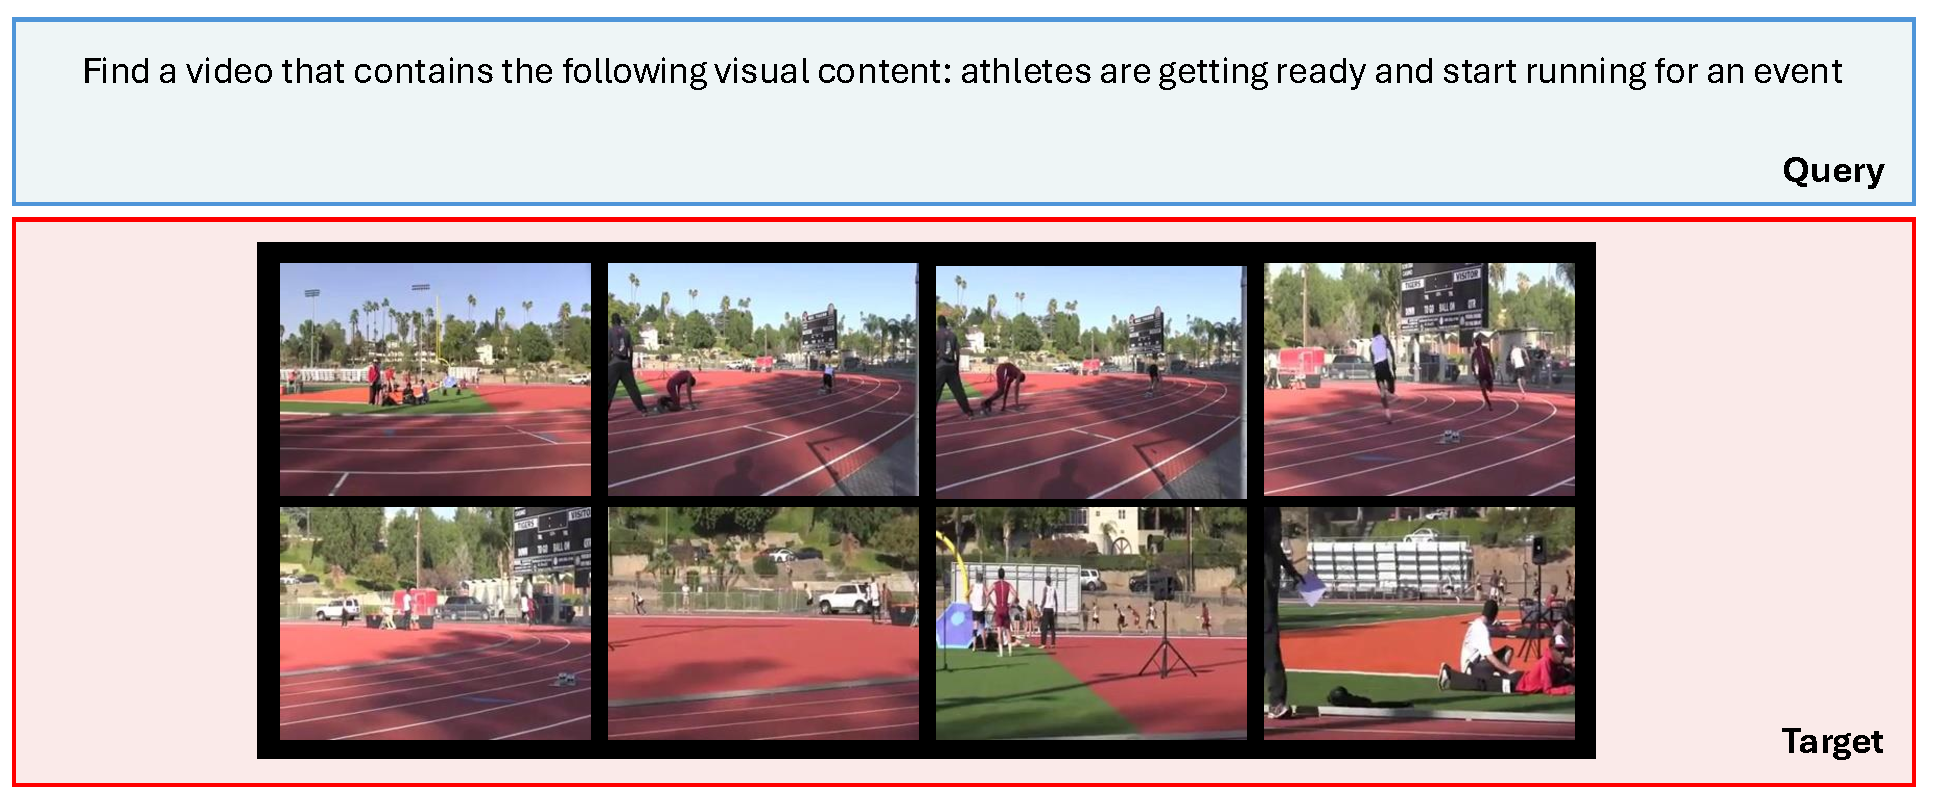
\includegraphics[width=\linewidth]{figures/dataset_example_figures/msrvtt_example.pdf}
%     \caption{An example of the video retrieval task on the video retrieval task in our benchmark.}
%     \label{fig:msrvtt_example}
% \end{figure}

% \begin{figure}[!h]
%     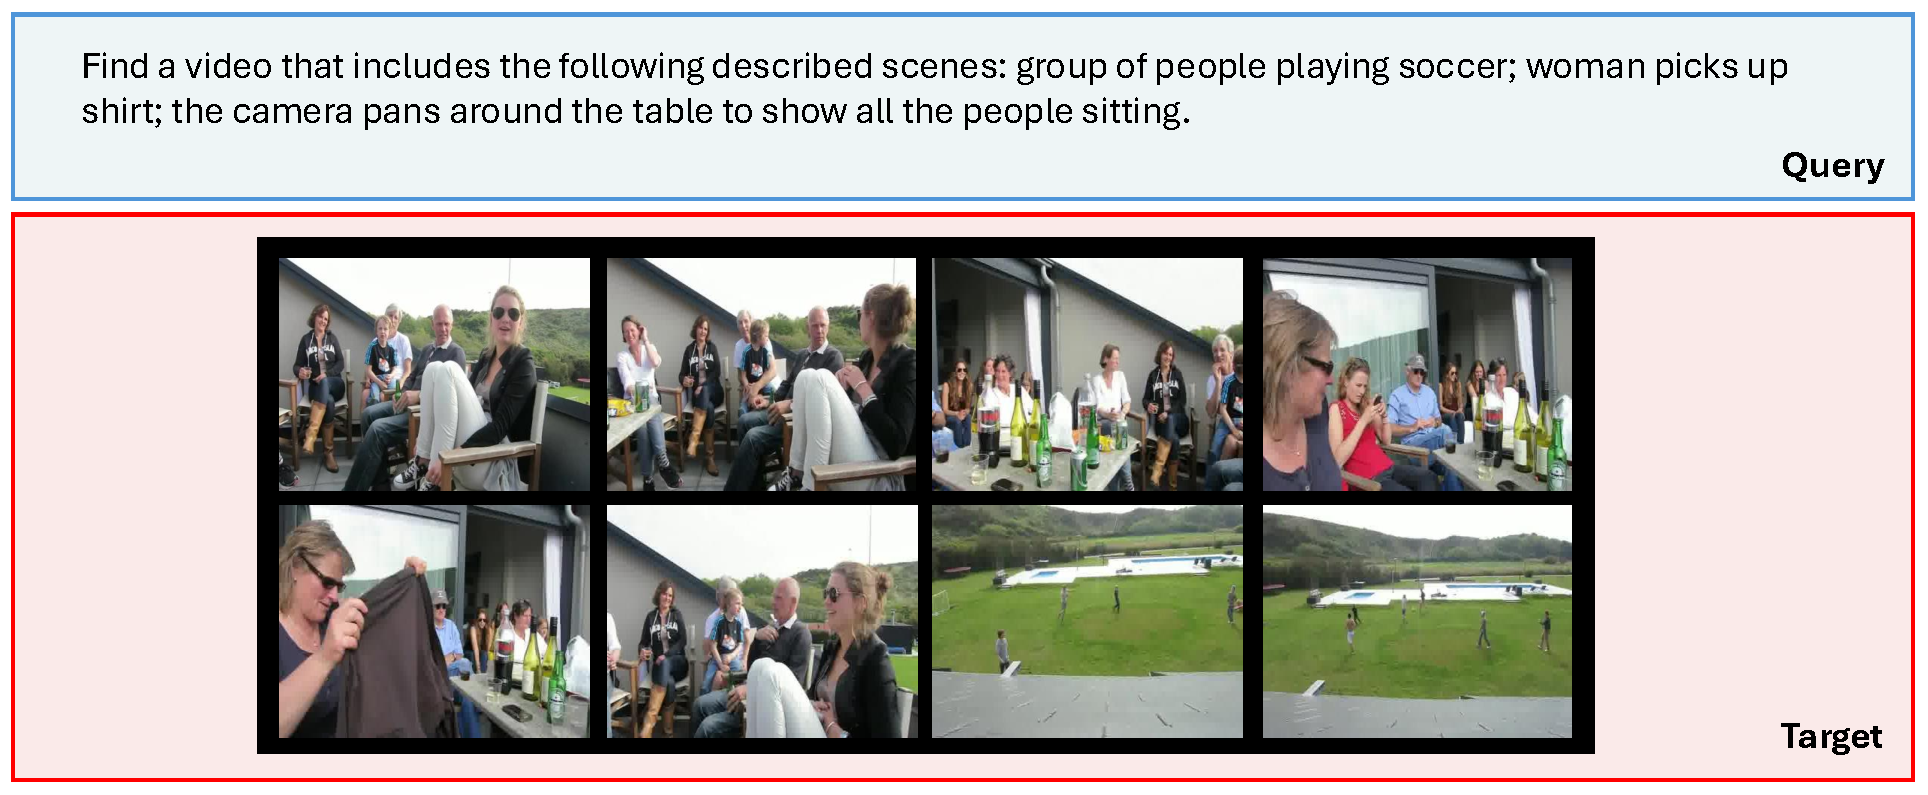
\includegraphics[width=\linewidth]{figures/dataset_example_figures/didemo_example.pdf}
%     \caption{An example of the video retrieval task on the DiDeMo task in our benchmark.}
%     \label{fig:didemo_example}
% \end{figure}

% \begin{figure}[!h]
%     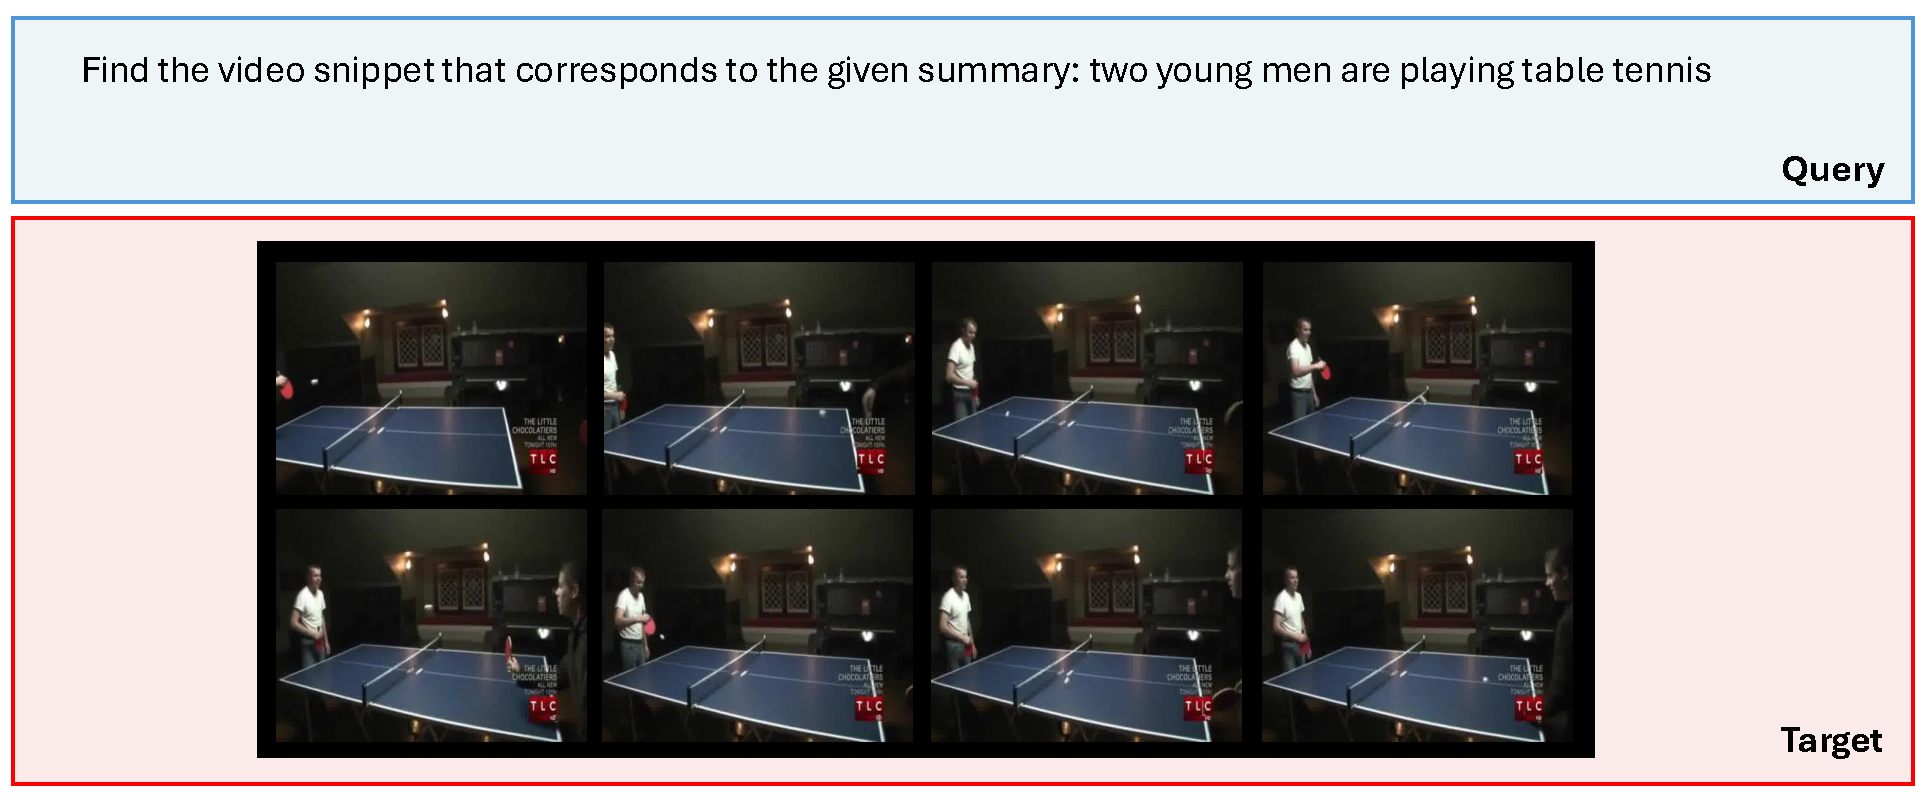
\includegraphics[width=\linewidth]{figures/dataset_example_figures/msvd_example.pdf}
%     \caption{An example of the video retrieval task on the MSVD task in our benchmark.}
%     \label{fig:msvd_example}
% \end{figure}


% \subsection{Additional Details of Training Data}
% \label{sec::appendix_training_data_details}



\subsection{Detailed Scores}
\label{sec::full_score_table}
\definecolor{avgcolor}{RGB}{235,245,255}     % light blue
\definecolor{icatcolor}{RGB}{255,240,220}    % light orange-peach
\definecolor{vcatcolor}{RGB}{235,255,235}    % light green
\definecolor{vdcatcolor}{RGB}{245,230,255}   % light purple


\begin{table}[!ht]
    \centering
    \renewcommand{\arraystretch}{0.8}
    \begin{adjustbox}{width=\textwidth}
    \begin{tabular}{l|cccccccc}
        \toprule
        ~ & ColPali v1.3 & GME-2B & GME-7B & LamRA-Qwen2 & LamRA-Qwen2.5 & VLM2Vec-2B & VLM2Vec-7B & VLM2Vec-V2.0 \\ 
        \midrule
        \rowcolor{avgcolor}
        Avg - All (78 tasks) & 46.0 & 54.1 & 57.8 & 40.4 & 47.4 & 47.0 & 52.3 & 58.0 \\ 
        \midrule
        \rowcolor{avgcolor}
        Avg - Image (36 tasks, Hit@1) & 34.9 & 51.9 & 56.0 & 54.1 & 52.4 & 59.7 & 65.5 & 64.9 \\ 
        \rowcolor{avgcolor}
        Avg - Video (18 tasks, Hit@1) & 28.2 & 33.6 & 38.4 & 35.0 & 33.6 & 28.6 & 33.7 & 34.6 \\ 
        \rowcolor{avgcolor}
        Avg - Visdoc (24 tasks, NDCG@5) & 75.8 & 72.7 & 75.2 & 23.9 & 50.2 & 41.6 & 46.4 & 65.4 \\
        \midrule
        \rowcolor{icatcolor}
        I-CLS (10) & 40.3 & 54.4 & 57.7 & 59.2 & 51.7 & 58.7 & 62.7 & 62.9 \\ 
        \rowcolor{icatcolor}
        I-QA (10) & 11.5 & 29.9 & 34.7 & 26.5 & 34.1 & 49.3 & 56.9 & 56.3 \\ 
        \rowcolor{icatcolor}
        I-RET (12) & 48.1 & 66.9 & 71.2 & 70.0 & 66.9 & 65.0 & 69.4 & 69.5 \\ 
        \rowcolor{icatcolor}
        I-VG (4) & 40.3 & 55.5 & 59.3 & 62.7 & 56.7 & 72.9 & 82.2 & 77.3 \\ 
        % \hdashline
        \rowcolor{vcatcolor}
        V-CLS (5) & 26.7 & 34.9 & 37.4 & 39.3 & 32.9 & 33.4 & 39.1 & 39.3 \\ 
        \rowcolor{vcatcolor}
        V-QA (5) & 37.8 & 42.0 & 50.4 & 42.6 & 42.6 & 30.5 & 30.0 & 34.3 \\ 
        \rowcolor{vcatcolor}
        V-RET (5) & 21.6 & 25.6 & 28.4 & 24.3 & 23.2 & 20.6 & 29.0 & 28.8 \\ 
        \rowcolor{vcatcolor}
        V-MR (3) & 25.5 & 31.1 & 37.0 & 32.8 & 37.2 & 30.7 & 38.9 & 36.8 \\ 
        % \hdashline
        \rowcolor{vdcatcolor}
        VD-Vidore-V1 (10) & 83.6 & 86.1 & 89.4 & 22.0 & 56.3 & 49.8 & 56.9 & 75.5 \\ 
        \rowcolor{vdcatcolor}
        VD-Vidore-V2 (4) & 52.0 & 54.0 & 55.6 & 11.5 & 33.3 & 13.5 & 9.4 & 44.9 \\ 
        \rowcolor{vdcatcolor}
        VD-VisRAG (6) & 81.1 & 82.5 & 85.0 & 37.4 & 58.2 & 51.8 & 59.1 & 79.4 \\ 
        \rowcolor{vdcatcolor}
        VD-OOD (4) & 43.1 & 43.1 & 44.4 & 21.0 & 40.1 & 33.5 & 38.1 & 39.4 \\ 
        \midrule
        
        ImageNet-1K & 42.4 & 58.3 & 64.6 & 72.3 & 58.9 & 77.5 & 80.1 & 80.8 \\ 
        N24News & 25.5 & 50.1 & 50.5 & 51.3 & 29.8 & 73.7 & 79.7 & 72.9 \\ 
        HatefulMemes & 50.6 & 52.5 & 53.6 & 49.0 & 51.3 & 58.3 & 69.7 & 56.3 \\ 
        VOC2007 & 69.8 & 75.9 & 80.3 & 80.1 & 78.7 & 74.3 & 80.7 & 85.0 \\ 
        SUN397 & 56.1 & 67.3 & 69.5 & 68.5 & 66.5 & 73.8 & 77.4 & 71.0 \\ 
        Place365 & 27.5 & 35.8 & 39.1 & 40.6 & 37.4 & 35.3 & 37.4 & 35.9 \\ 
        ImageNet-A & 14.9 & 28.8 & 41.2 & 47.0 & 36.3 & 50.9 & 58.1 & 47.4 \\ 
        ImageNet-R & 64.6 & 78.6 & 83.9 & 88.5 & 77.0 & 84.7 & 73.9 & 89.3 \\ 
        ObjectNet & 45.6 & 70.6 & 69.0 & 66.4 & 59.4 & 37.1 & 40.1 & 65.2 \\ 
        Country211 & 6.0 & 26.5 & 24.8 & 28.3 & 21.7 & 21.5 & 29.8 & 25.2 \\ 
        OK-VQA & 9.4 & 29.9 & 33.2 & 37.8 & 39.9 & 48.5 & 56.8 & 51.5 \\ 
        A-OKVQA & 6.6 & 18.6 & 21.0 & 27.0 & 34.1 & 39.5 & 47.3 & 43.6 \\ 
        DocVQA & 11.3 & 29.8 & 41.4 & 22.3 & 37.1 & 82.5 & 89.7 & 90.1 \\ 
        InfographicsVQA & 5.0 & 11.6 & 20.3 & 16.5 & 23.7 & 47.7 & 60.0 & 58.8 \\ 
        ChartQA & 5.7 & 13.4 & 17.8 & 11.7 & 15.0 & 42.3 & 56.9 & 47.4 \\ 
        Visual7W & 6.1 & 16.2 & 22.2 & 19.6 & 24.6 & 51.2 & 52.7 & 52.9 \\ 
        ScienceQA & 16.3 & 27.3 & 28.0 & 26.3 & 31.3 & 30.7 & 38.5 & 38.2 \\ 
        VizWiz & 27.6 & 37.0 & 39.0 & 32.0 & 32.0 & 38.6 & 39.9 & 43.3 \\ 
        GQA & 8.3 & 75.1 & 76.9 & 38.5 & 57.4 & 48.3 & 55.1 & 64.9 \\ 
        TextVQA & 18.8 & 39.7 & 46.8 & 33.0 & 46.1 & 63.3 & 71.6 & 72.2 \\ 
        VisDial & 41.2 & 48.1 & 60.8 & 61.3 & 62.5 & 74.3 & 81.9 & 82.7 \\ 
        CIRR & 8.2 & 44.2 & 54.9 & 51.7 & 44.7 & 46.8 & 51.1 & 57.5 \\ 
        VisualNews\_t2i & 50.1 & 74.7 & 79.7 & 70.4 & 70.1 & 73.1 & 80.5 & 74.5 \\ 
        VisualNews\_i2t & 47.6 & 78.3 & 83.6 & 83.9 & 74.2 & 73.7 & 81.2 & 78.2 \\ 
        MSCOCO\_t2i & 59.2 & 68.1 & 71.2 & 72.2 & 65.7 & 73.4 & 77.2 & 75.3 \\ 
        MSCOCO\_i2t & 49.9 & 63.1 & 57.7 & 73.7 & 71.1 & 68.5 & 73.9 & 71.4 \\ 
        NIGHTS & 65.5 & 67.0 & 67.6 & 65.6 & 64.4 & 66.3 & 67.6 & 68.6 \\ 
        WebQA & 53.8 & 88.8 & 91.4 & 81.0 & 85.7 & 85.9 & 88.3 & 90.6 \\ 
        FashionIQ & 5.9 & 32.9 & 37.8 & 42.0 & 33.4 & 14.0 & 17.1 & 19.5 \\ 
        Wiki-SS-NQ & 80.5 & 73.9 & 78.2 & 69.7 & 67.0 & 54.2 & 62.3 & 66.9 \\ 
        OVEN & 50.0 & 72.3 & 75.1 & 82.0 & 84.8 & 68.3 & 66.5 & 64.3 \\ 
        EDIS & 64.7 & 91.8 & 96.0 & 85.9 & 78.7 & 81.2 & 85.7 & 84.1 \\ 
        MSCOCO & 36.7 & 28.6 & 31.4 & 44.8 & 36.0 & 66.5 & 75.7 & 67.1 \\ 
        RefCOCO & 64.5 & 55.9 & 60.9 & 62.8 & 57.1 & 80.9 & 87.6 & 87.1 \\ 
        RefCOCO-Matching & 3.9 & 73.3 & 78.4 & 75.7 & 82.6 & 75.7 & 84.6 & 85.8 \\ 
        Visual7W-Pointing & 56.1 & 64.1 & 66.5 & 67.3 & 51.2 & 68.3 & 81.0 & 69.2 \\ 
        \midrule
        
        K700 & 23.4 & 35.2 & 39.7 & 42.3 & 32.1 & 31.4 & 35.5 & 38.0 \\ 
        SmthSmthV2 & 25.1 & 29.9 & 30.6 & 36.3 & 25.3 & 30.9 & 32.1 & 42.8 \\ 
        HMDB51 & 24.8 & 43.4 & 47.9 & 40.5 & 33.8 & 33.8 & 42.2 & 40.9 \\ 
        UCF101 & 49.4 & 52.4 & 54.7 & 60.4 & 53.0 & 57.5 & 61.8 & 60.0 \\ 
        Breakfast & 10.9 & 13.6 & 14.3 & 16.9 & 20.1 & 13.4 & 23.8 & 14.8 \\ 
        MVBench & 33.7 & 37.5 & 46.6 & 37.2 & 37.6 & 30.5 & 28.5 & 33.7 \\ 
        Video-MME & 30.6 & 34.3 & 39.2 & 34.1 & 35.1 & 26.9 & 27.8 & 30.7 \\ 
        NExTQA & 35.2 & 39.5 & 53.6 & 43.7 & 44.9 & 20.3 & 20.3 & 20.9 \\ 
        EgoSchema & 38.4 & 40.8 & 46.8 & 44.8 & 47.0 & 25.4 & 21.8 & 34.0 \\ 
        ActivityNetQA & 51.3 & 58.0 & 65.6 & 53.2 & 48.5 & 49.6 & 51.4 & 52.3 \\ 
        DiDeMo & 22.8 & 22.0 & 26.4 & 24.8 & 22.8 & 19.4 & 29.3 & 30.4 \\ 
        MSR-VTT & 17.6 & 27.3 & 31.8 & 22.1 & 25.0 & 25.2 & 34.5 & 28.3 \\ 
        MSVD & 45.4 & 47.6 & 49.7 & 46.1 & 41.9 & 38.2 & 46.7 & 48.1 \\ 
        VATEX & 16.7 & 23.0 & 24.9 & 19.1 & 18.7 & 16.2 & 25.5 & 26.5 \\ 
        YouCook2 & 5.3 & 7.9 & 9.1 & 9.2 & 7.5 & 4.1 & 9.0 & 10.6 \\ 
        QVHighlight & 19.9 & 43.6 & 59.5 & 53.8 & 60.9 & 44.2 & 57.7 & 49.4 \\ 
        Charades-STA & 29.0 & 14.9 & 14.0 & 10.9 & 18.8 & 13.6 & 19.8 & 20.2 \\ 
        MomentSeeker & 29.3 & 37.1 & 39.3 & 35.9 & 33.3 & 35.4 & 41.0 & 42.9 \\ 
        % MomentSeeker (1.8k queries, with dups) & 27.6 & 34.8 & 37.4 & 33.8 & 31.8 & 34.4 & 39.3 & 40.8 \\ 
        \midrule
        
        ViDoRe\_arxivqa & 81.7 & 82.8 & 86.9 & 10.8 & 53.0 & 48.9 & 60.2 & 80.6 \\ 
        ViDoRe\_docvqa & 56.6 & 53.1 & 57.5 & 19.1 & 25.4 & 27.0 & 34.7 & 44.9 \\ 
        ViDoRe\_infovqa & 84.9 & 90.2 & 91.6 & 46.3 & 72.3 & 67.2 & 70.4 & 83.7 \\ 
        ViDoRe\_tabfquad & 86.9 & 93.3 & 94.6 & 42.8 & 66.1 & 62.6 & 78.2 & 89.2 \\ 
        ViDoRe\_tatdqa & 70.9 & 69.9 & 74.1 & 11.4 & 25.9 & 19.8 & 27.6 & 43.8 \\ 
        ViDoRe\_shiftproject & 75.1 & 89.5 & 96.8 & 12.0 & 27.3 & 41.8 & 38.6 & 60.8 \\ 
        ViDoRe\_artificial\_intelligence & 95.7 & 97.5 & 99.6 & 10.3 & 72.0 & 55.0 & 67.7 & 88.5 \\ 
        ViDoRe\_energy & 94.7 & 91.9 & 95.3 & 24.8 & 65.2 & 59.1 & 60.4 & 86.5 \\ 
        ViDoRe\_government\_reports & 93.6 & 94.6 & 98.8 & 16.4 & 72.2 & 57.1 & 61.8 & 85.0 \\ 
        ViDoRe\_healthcare\_industry & 95.9 & 98.7 & 99.3 & 25.9 & 83.8 & 59.6 & 69.9 & 92.2 \\ 
        ViDoRe\_esg\_reports\_human\_labeled\_v2 & 51.3 & 61.0 & 63.4 & 7.6 & 33.0 & 12.6 & 6.8 & 45.6 \\ 
        ViDoRe\_biomedical\_lectures\_v2\_multilingual & 54.7 & 54.0 & 49.5 & 13.3 & 35.9 & 7.4 & 5.1 & 44.3 \\ 
        ViDoRe\_economics\_reports\_v2\_multilingual & 49.0 & 50.2 & 54.2 & 19.1 & 31.9 & 13.9 & 13.9 & 43.0 \\ 
        ViDoRe\_esg\_reports\_v2\_multilingual & 52.9 & 50.7 & 55.4 & 5.9 & 32.5 & 20.1 & 11.9 & 46.6 \\ 
        VisRAG\_ArxivQA & 80.9 & 82.0 & 87.4 & 2.0 & 37.7 & 41.8 & 52.6 & 76.9 \\ 
        VisRAG\_ChartQA & 78.2 & 79.9 & 81.9 & 41.3 & 65.9 & 57.9 & 70.2 & 84.4 \\ 
        VisRAG\_MP-DocVQA & 86.8 & 84.4 & 89.2 & 33.4 & 54.5 & 43.2 & 52.8 & 71.8 \\ 
        VisRAG\_SlideVQA & 95.0 & 93.4 & 94.5 & 56.5 & 76.5 & 74.0 & 72.8 & 91.5 \\ 
        VisRAG\_InfoVQA & 85.7 & 91.4 & 93.5 & 56.3 & 73.3 & 70.7 & 72.0 & 85.7 \\ 
        VisRAG\_PlotQA & 60.3 & 64.1 & 63.4 & 34.6 & 41.2 & 23.4 & 34.4 & 66.1 \\ 
        % TODO: 20251105 need to update scores with the fixed version
        ViDoSeek-page & 22.2 & 21.6 & 23.2 & 11.3 & 23.1 & 17.7 & 22.3 & 21.9 \\ 
        ViDoSeek-doc & 83.7 & 83.6 & 83.9 & 37.1 & 80.3 & 74.3 & 77.8 & 80.2 \\ 
        MMLongBench-page & 14.2 & 15.8 & 16.2 & 8.0 & 13.5 & 9.6 & 11.8 &  11.9 \\
        MMLongBench-doc & 52.5 & 51.4 & 54.3 & 27.6 & 43.5 & 32.6 & 40.5 & 43.7 \\         
    \bottomrule
    \end{tabular}
    \end{adjustbox}
\caption{
Performance comparison of various models on the full \benchmark benchmark, covering 78 tasks across image, video, and visual document modalities. Numbers in parentheses represent the task count for each category.}
\label{tab:full_score}
\end{table}



\clearpage

\subsection{Updated Results on the MMEB-V2 Benchmark}
Since the release of the MMEB series benchmarks, they have become widely adopted as standard evaluations for MLLM embeddings. As of December 2025, more than 50 models have been evaluated on MMEB-V1 and over 30 models on MMEB-V2. In this appendix, we include additional results from several recent state-of-the-art multimodal embedding models evaluated on the MMEB-V2 benchmark.


\begin{table*}[t]
\centering
\small
\setlength{\tabcolsep}{6pt}
\begin{tabular}{c l c c c c c}
\toprule
\textbf{Rank} & \textbf{Model} & \textbf{Size (B)} & \textbf{Overall} & \textbf{Image} & \textbf{Video} & \textbf{VisDoc} \\
\midrule
1  & seed1.6-embedding-1215        & --    & 75.59 & 77.99 & 67.74 & 77.88 \\
2  & WeMM-Embedding-8B             & 8.77  & 74.42 & 78.09 & 63.24 & 77.30 \\
3  & IFM-TTE-7B                    & 8.29  & 74.07 & 77.90 & 59.19 & 79.48 \\
4  & WeMM-Embedding-2B             & 2.13  & 71.67 & 76.08 & 58.67 & 74.81 \\
5  & RzenEmbed-v2-7B               & 8.29  & 71.61 & 75.92 & 55.73 & 77.06 \\
6  & seed-1.6-embedding             & --    & 71.27 & 77.78 & 55.34 & 73.44 \\
7  & RzenEmbed-v1-7B               & 8.29  & 68.88 & 73.60 & 48.87 & 76.80 \\
8  & Ops-MM-embedding-v1-7B        & 8.29  & 67.61 & 72.72 & 53.76 & 70.34 \\
9  & UME-R1-7B                     & 8.29  & 64.50 & 71.25 & 47.50 & 67.13 \\
10 & RzenEmbed-v1-2B               & 2.21  & 64.36 & 68.53 & 42.62 & 74.41 \\
11 & Ops-MM-embedding-v1-2B        & 2.21  & 63.44 & 69.03 & 47.56 & 66.96 \\
12 & interestFM-UIR-CAFe-7B        & 8.03  & 60.63 & 67.56 & 42.40 & 63.92 \\
13 & UME-R1-2B                     & 2.21  & 60.11 & 66.56 & 42.23 & 63.86 \\
14 & UniME-V2-LLaVA-OneVision-7B   & 8.03  & 59.56 & 71.77 & 39.01 & 56.68 \\
15 & VLM2Vec-V2.0-Qwen2VL-2B       & 2.21  & 58.02 & 64.85 & 34.58 & 65.36 \\
\bottomrule
\end{tabular}
\caption{Leaderboard results on the MMEB-V2 benchmark as of December 2025. Scores are reported for overall performance as well as for modality-specific subsets, including Image, Video, and VisDoc.
}
\label{tab:mmeb_v2_leaderboard}
\end{table*}



\clearpage

\subsection{Significance Evaluation of Modality Mixing Strategies}
\label{sec:significance_test}
\begin{table}[t]
\centering
\small
\setlength{\tabcolsep}{4pt}
\renewcommand{\arraystretch}{1.2}

\begin{tabular}{
  l
  S[table-format=+2.2] c
  S[table-format=+2.2] c
  S[table-format=+2.2] c
  S[table-format=+2.2] c}
\toprule
\textbf{Training Data Configuration} &
\multicolumn{2}{c}{\textbf{Image $\Delta$}} &
\multicolumn{2}{c}{\textbf{Video $\Delta$}} &
\multicolumn{2}{c}{\textbf{VisDoc $\Delta$}} &
\multicolumn{2}{c}{\textbf{Global $\Delta$}} \\
\cmidrule(lr){1-1}\cmidrule(lr){2-3}\cmidrule(lr){4-5}\cmidrule(lr){6-7}\cmidrule(lr){8-9}
Image 200K (Baseline) &
\multicolumn{2}{c}{--} &
\multicolumn{2}{c}{--} &
\multicolumn{2}{c}{--} &
\multicolumn{2}{c}{--} \\

Image 100K + ColPali 100K &
-1.74 &      &
-0.02 &      &
+7.76 & ***  &
+1.58 & *    \\

Image 100K + VideoCap 100K &
-2.52 & ***  &
-0.89 &      &
-0.36 &      &
-1.48 & ***  \\

Image 100K + ColPali 50K + VideoCap 50K &
-1.55 & **   &
+1.09 & *    &
+6.69 & ***  &
+1.59 & **   \\

All Sources 200K &
-2.13 & **   &
-0.84 &      &
+10.19 & *** &
+1.96 & *    \\
\bottomrule
\end{tabular}

\vspace{4pt}
\caption{Task-level significance evaluation of different modality mixing strategies compared to the Image 200K baseline. Listed values indicate the mean performance change across 78 MMEB-V2 tasks, with positive values reflecting consistent gains. Statistical reliability is assessed using paired $t$-tests: * $p < 0.05$, ** $p < 0.01$, *** $p < 0.001$.}
\label{tab:stat_significance}
\end{table}



To rigorously assess the generalization impact of multimodal training configurations (Section~\ref{sec:modality_generalization}; Table~\ref{tab:data_mix_t2}), we conduct a task-level paired $t$-test to evaluate statistical significance. Instead of treating individual queries as independent observations—which would artificially inflate significance due to large sample counts—we treat each dataset (task) as one independent sample ($N=78$ tasks). For each ablation model $M$, we compute a paired difference vector $D=[\text{Score}_{M,1}-\text{Score}_{\text{Base},1},\dots,\text{Score}_{M,N}-\text{Score}_{\text{Base},N}]$, comparing its performance to that of the Image-only baseline on a per-task basis. We then test the null hypothesis that the mean of $D$ is zero, where the sign of the mean difference reflects improvement or degradation, and the $p$-value indicates whether the effect is statistically reliable across the full task distribution.

The significance results in Table~\ref{tab:stat_significance} confirm the key observations from Section~\ref{sec:modality_generalization}. In particular, \textbf{effective modality mixing requires both high-quality data and modality compatibility}: adding curated VisDoc supervision (e.g., \texttt{ColPali}) leads to statistically significant gains, whereas incorporating noisier video supervision (\texttt{VideoCap}) can negatively affect performance. Furthermore, \textbf{the two full Image + VisDoc + Video mixtures deliver the strongest global improvements}, highlighting that broader modality coverage is most beneficial when additional modalities are carefully selected and curated.




\clearpage

\subsection{Example Cases}
\label{sec:example_cases}

\begin{figure}[!ht]
  \centering
    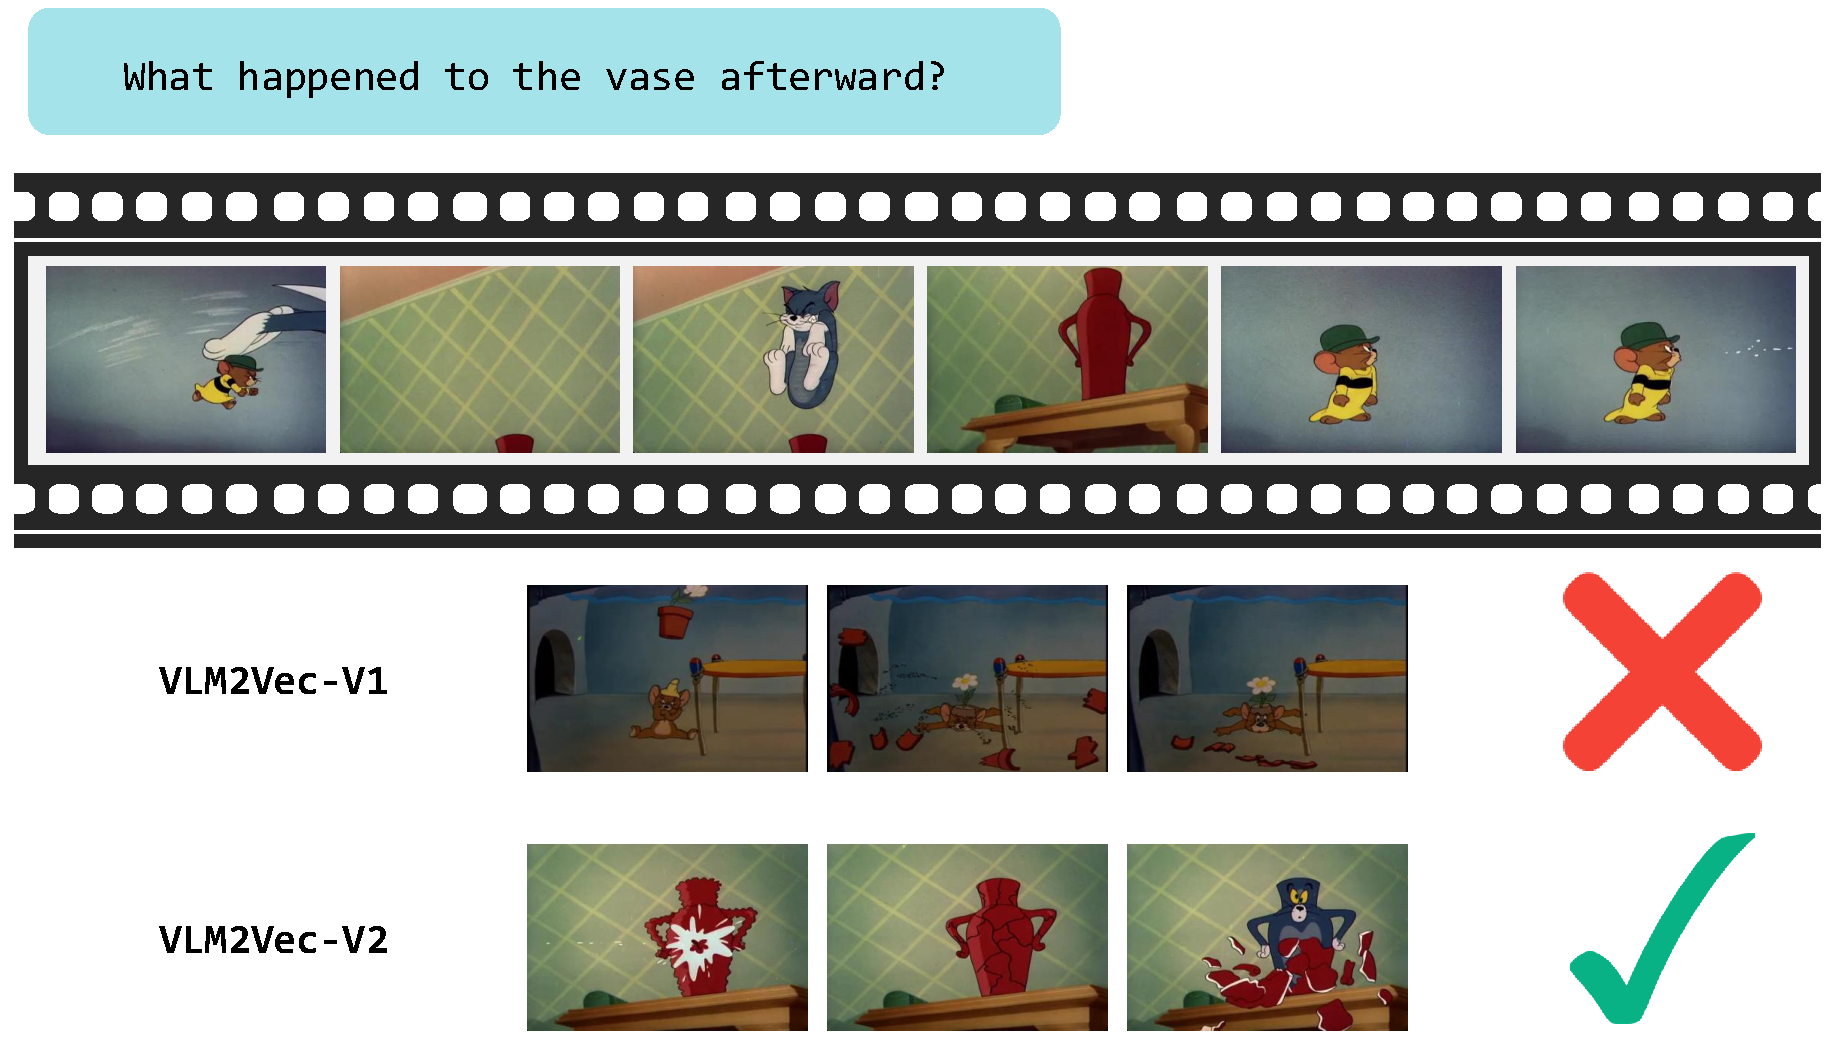
\includegraphics[width=\linewidth]{figures/vlm2vec_example1.pdf}
    \caption{Example of improved video understanding in \model over \vlmvec.}
    \vspace{-3ex}
    \label{fig:example_1}
\end{figure}

\begin{figure}[!ht]
  \centering
    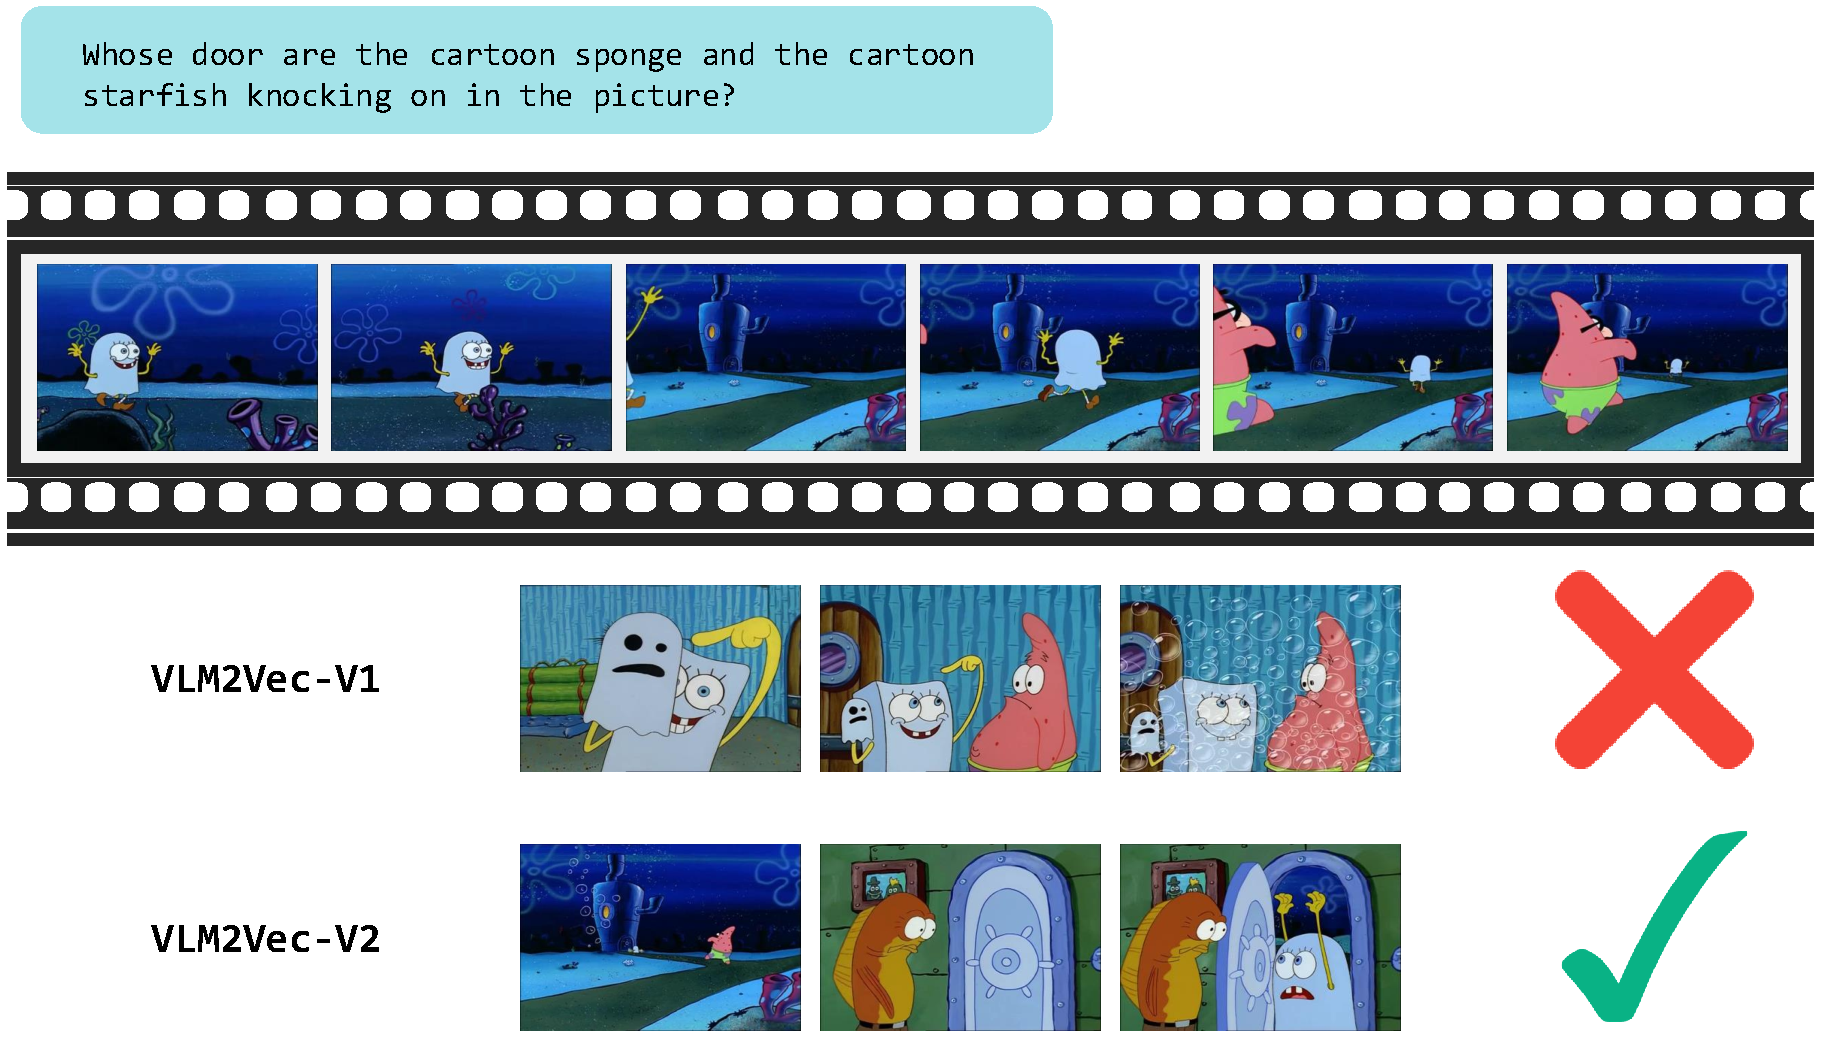
\includegraphics[width=\linewidth]{figures/vlm2vec_example2.pdf}
    \caption{Example of improved video understanding in \model over \vlmvec.}
    \vspace{-3ex}
    \label{fig:example_2}
\end{figure}

\begin{figure}[!ht]
  \centering
    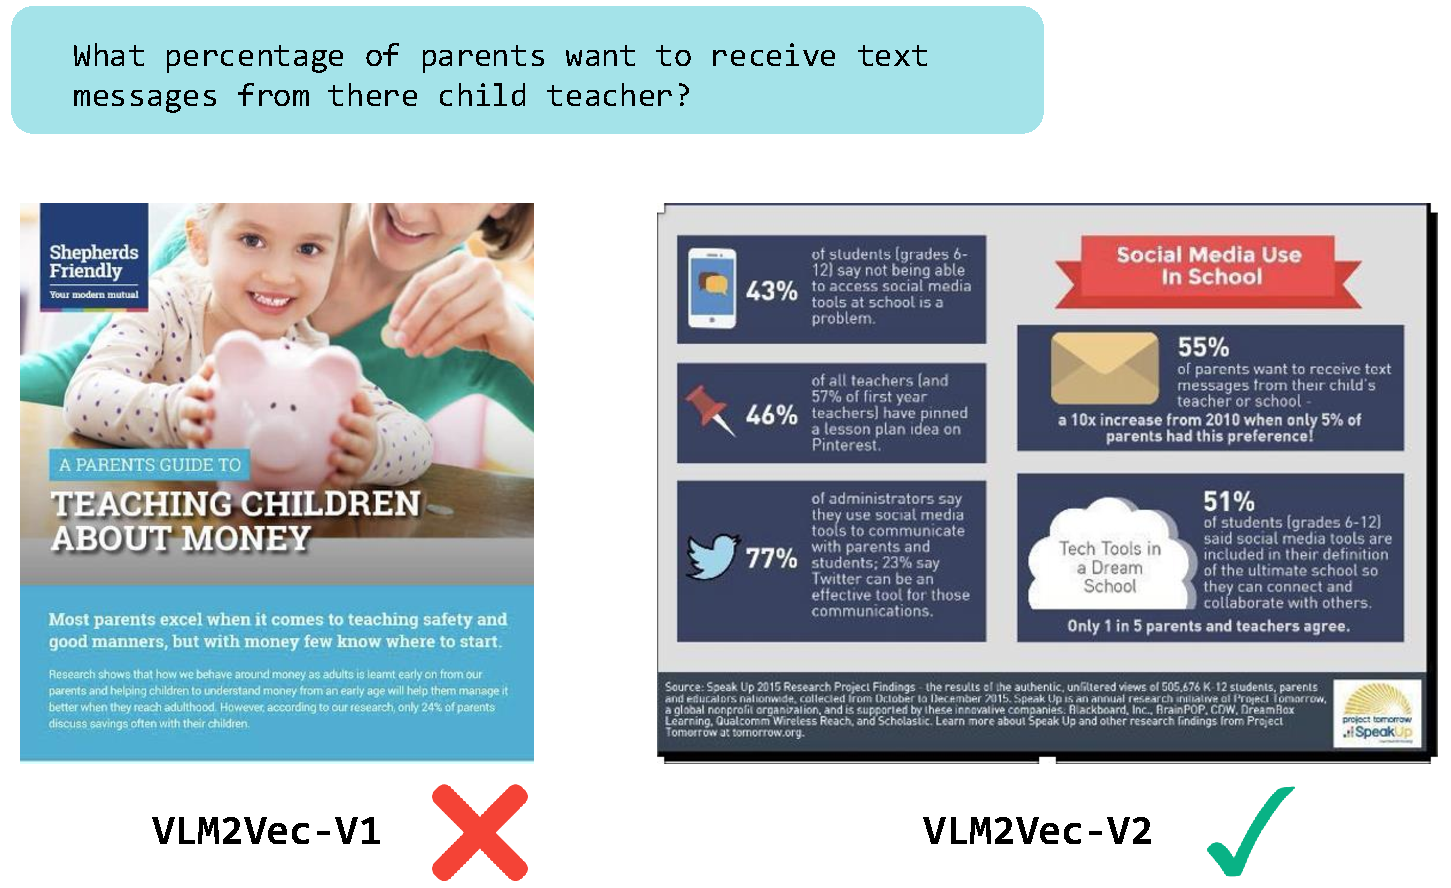
\includegraphics[width=\linewidth]{figures/vlm2vec_example3.pdf}
    \caption{Example of improved document understanding in \model over \vlmvec. The images are cropped for clearer presentation.}
    \vspace{-3ex}
    \label{fig:example_3}
\end{figure}

\begin{figure}[!ht]
  \centering
    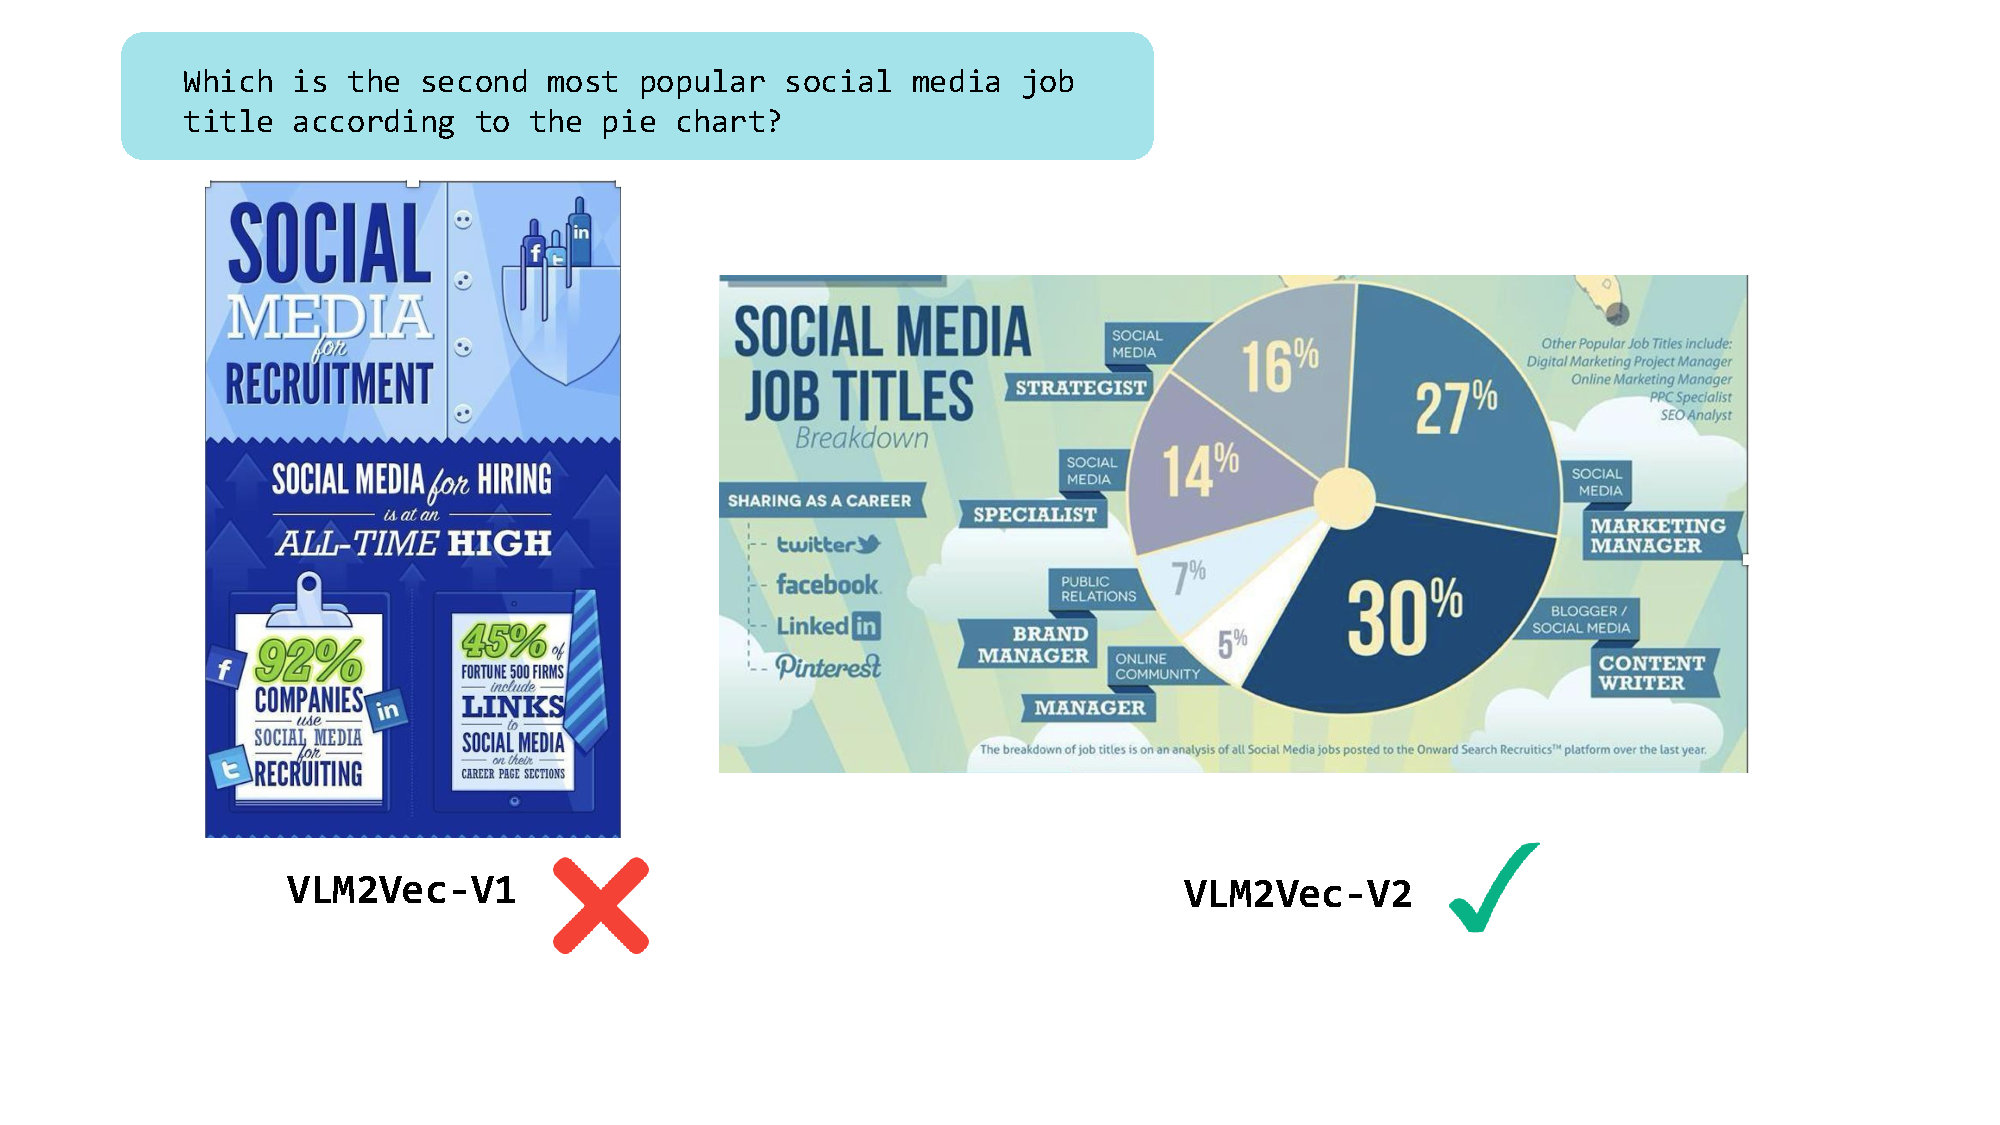
\includegraphics[width=\linewidth]{figures/vlm2vec_example4.pdf}
    \caption{Example of improved document understanding in \model over \vlmvec. The images are cropped for clearer presentation.}
    \vspace{-3ex}
    \label{fig:example_4}
\end{figure}
